\documentclass[UTF8]{mcmthesis}
    % \usepackage{ctex}           % 暂时需要中文时添加, 最后注释掉即可
    \mcmsetup {
        tcn = 2505974, problem = B,    %% tcn is team control number
        titleinsummary = true,             %% title appears on summary sheet
    }
    \usepackage{pdfpages}

\usepackage{hyperref}
\hypersetup{
	colorlinks=true,
	linkcolor=black
}
    % 调整 \item 的间距 
    \usepackage{paralist}
    \usepackage{enumitem}

        \let\itemize\compactitem
        \let\enditemize\endcompactitem
        \let\enumerate\compactenum
        \let\endenumerate\endcompactenum
        \let\description\compactdesc
        \let\enddescriprion\endcompactdesc
    % 调整公式和正文的间距 (公式和正文更紧凑)
    \makeatletter
    \renewcommand\normalsize {
        % \@setfontsize\normalsize\@xpt\@xiipt
        \abovedisplayskip 5\p@ \@plus2\p@ \@minus5\p@
        \abovedisplayshortskip \z@ \@plus3\p@
        \belowdisplayshortskip 5\p@ \@plus3\p@ \@minus3\p@
        \belowdisplayskip \abovedisplayskip
        \let\@listi\@listI
    }
    \makeatother

    % \renewcommand{\baselinestretch}{1.2}      % 行间距
    \setlength{\parskip}{0.5em}                 % 段间距

    \usepackage{tikz}
        \usetikzlibrary{arrows} % 按需要添加扩展

    % 一般默认字体就好
    % \usepackage{mathptmx}     %% 数学公式罗马字体,对公式和正文都起作用
    % \usepackage{txfonts}      %% 数学公式罗马字体,对公式和正文都起作用
    % \usepackage{mathpazo}     %% COMAP 官方版物字体,对公式和正文都起作用
    % 一些重命名 ↓
    % \providecommand{\diff}{\mathop{}\!\mathrm{d}} %% 微分符号,正体 d
    % \providecommand{\me}{\mathrm{e}}              %% 无理数,正体 e
    % \providecommand{\mi}{\mathrm{i}}              %% 虚数单位,正体 i

    %% 设置目录节标题后加点
    \usepackage[titles]{tocloft}
    \renewcommand\cftsecdotsep{\cftdotsep}
    \renewcommand{\appendixpagename}{\Large\bfseries Appendices}

    %% 定制 Synopsis 页目录
    %% 根据需要把 Synopsis 改为 Memo or Handout 等等
    \fancypagestyle{Synopsis} {
        \fancyhf{}
        \lhead{\sffamily \team}
        \rhead{\sffamily Synopsis}
    }
    \title{\bfseries SaberArcherLancer}  % 题目
  
\begin{document}
    \begin{summary}
        \begin{align*}
            \textbf{Summary}
        \end{align*}
        \hspace*{2em} Juneau, Alaska, as a world-renowned tourist destination, faces significant challenges in balancing its economic dependence on tourism with environmental sustainability and community well-being. With an influx of over 1.6 million cruise ship passengers annually, the city has experienced severe overcrowding, environmental degradation, and strained infrastructure. This paper aims to build a sustainable tourism model to mitigate these issues, optimize resource allocation, and ensure long-term ecological and economic stability.

        In this study, we employed a variety of advanced mathematical models and techniques, including \textbf{multi-objective programming}, \textbf{SLSQP optimization algorithm}, and the \textbf{entropy weight method}. Our analysis was informed by a comprehensive review of relevant literature and relied on reliable data sources, ensuring both rigor and credibility. The integration of these methods allowed us to systematically evaluate and address the complexities of sustainable tourism management.

        To address the first question, we developed a multi-objective programming model comprising three hierarchical layers. The top layer optimizes overarching goals such as maximizing economic gain, minimizing environmental degradation, and enhancing resident satisfaction. The middle layer quantifies these goals using key performance indicators, and the bottom layer incorporates decision variables such as the number of tourists, tax rates, and revenue distribution. This layered structure ensures a holistic approach to sustainable tourism planning.

        For the second question, we adapted our model to Beijing, a city facing overtourism challenges exacerbated by severe air pollution. By integrating Beijing's unique environmental constraints, such as smog levels and public health considerations, we refined the model to reflect local conditions. Additionally, we proposed strategies to promote less-visited attractions within Beijing, encouraging a more balanced distribution of tourists and alleviating pressure on overcrowded sites.

        In our sensitivity analysis, we rigorously followed a structured process to evaluate the robustness of our model under varying conditions. This analysis identified the most critical factors influencing sustainable tourism outcomes, such as environmental recovery rates, tourist spending, and governance efficiency, ensuring the reliability of our recommendations.

        Finally, as part of this paper, we have included a concise and meticulously crafted memo addressed to the tourist council of Juneau. This memo summarizes our findings, highlights the predicted effects of various measures, and provides actionable advice on optimizing outcomes for a sustainable tourism industry.
        

    
        \vspace{2em}
        \noindent\textbf{Key Words: } Sustainable Tourism; Multi-objective Optimization  
    \end{summary}

    \maketitle
    \tableofcontents

    \setcounter{page}{1}
    \section{Introduction}
        \subsection{Problem Background}
            \hspace*{2em}Juneau, one of the most captivating tourist destinations in the United States, attracts visitors from around the world with its unique charm and natural beauty. Though only accessible by air and sea, the city’s allure remains irresistible to travelers.
            However, while tourism brings significant economic benefits, it also presents risks due to the fragile environmental resources and the potential for irreversible degradation. With a population of just under 30,000 residents, Juneau is already grappling with the strain of millions of tourists each year. To mitigate these impacts, immediate measures are needed to ensure sustainable tourism and enhance both the safety and well-being of the local community.
            
            Therefore, it is crucial to assess the true impact of tourism on the city. By adopting a science-based and rational approach, we can foster economic growth while preserving Juneau’s biodiversity and ecological integrity. Policymakers and the tourist council will benefit from reliable methods to measure how best to manage visitor numbers and allocate public funds to support community programs.
            
            In this paper, we will focus on key factors that influence sustainable tourism, examining their impact on key indicators. Additionally, based on our findings, we will provide long-term, generalized management recommendations that can be applied to other destinations facing overtourism challenges.

            \begin{figure}[htbp]
                \centering
                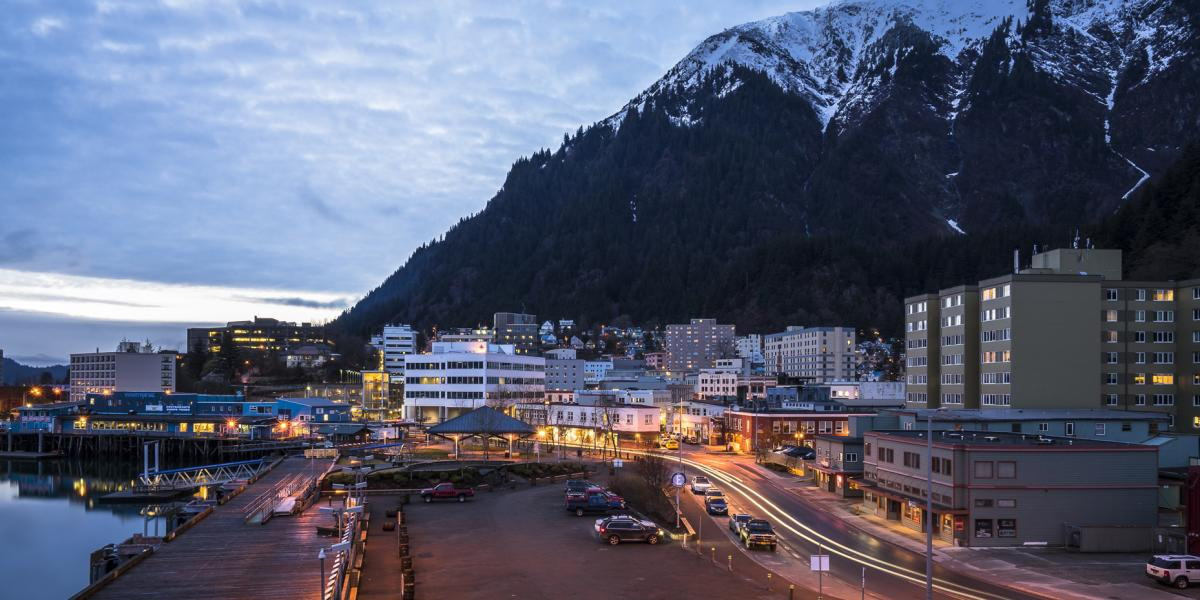
\includegraphics[width=8cm]{figure1.png}
                \caption{Dawn View of Juneau}
            \end{figure}
        
        \subsection{Restatement of the Problem}
        \hspace*{2em}Juneau is a famous toursism cities with many complexities and risks. Through in-depth analysis and research on the factors of the problem, combined with the specific constraints given, the restate of the objectives can be expressed as follows:


   
           \textbf{Objective 1:} Develop a comprehensive model to evaluate and optimize tourism management strategies. This model will consider variables such as visitor caps, revenue allocation, environmental preservation, and community well-being. Additionally, it will include a sensitivity analysis to prioritize factors most critical to sustainable tourism.

            
           \textbf{Objective 2:}Project and assess the long-term ecological, economic, and social outcomes of the proposed sustainable tourism model in Juneau. Evaluate how the implementation of these strategies will balance tourism growth with environmental and community health.

           
           \textbf{Objective 3:} Demonstrate how the developed model can be adapted to other tourist destinations impacted by overtourism. Provide actionable recommendations tailored to different locations to promote balanced tourism and optimize resource utilization.
           
           \subsection{Overview of Our Works}
           \hspace*{2em} Based on the comprehensive review of the existing reports and data, our work mainly includes the following:
           
           \begin{enumerate}
               \item \textbf{Firstly}, we begin by building a model to evaluate the \textbf{environmental status} and quantify its contributing factors. The environmental status is estimated by the area of one of the most significant ecosystems--\textbf{glaciers}.
               
               \item \textbf{Secondly}, we develop an \textbf{assessment model} that incorporates \textbf{economic gain} as a key variable. Additionally, we introduce a method to re-evaluate the \textbf{satisfaction of residents} as another critical factor. Through computation, we successfully quantified \textbf{G (economic gain)}, \textbf{E (environmental status)}, and \textbf{S (satisfaction index)}.
               
               \item \textbf{Furthermore}, we conduct a \textbf{multi-objective programming analysis} to optimize all considered factors, while including \textbf{necessary constraints}. This allows us to obtain \textbf{reasonable values} that can guide the enactment of sustainable management strategies.
               
               \item \textbf{Finally}, we adapt our model to \textbf{Beijing} and \textbf{Vatican}, two tourist destinations impacted by overtourism. By analyzing their specific features, we identified their \textbf{similarities and differences}. From a sectoral perspective, we utilized the same model to evaluate the \textbf{sustainable tourism conditions} for these two cities.
           \end{enumerate}
           
           
            \begin{figure}[htbp]
 
                \hspace{-1cm} % Adjust this value to move the image left or right
                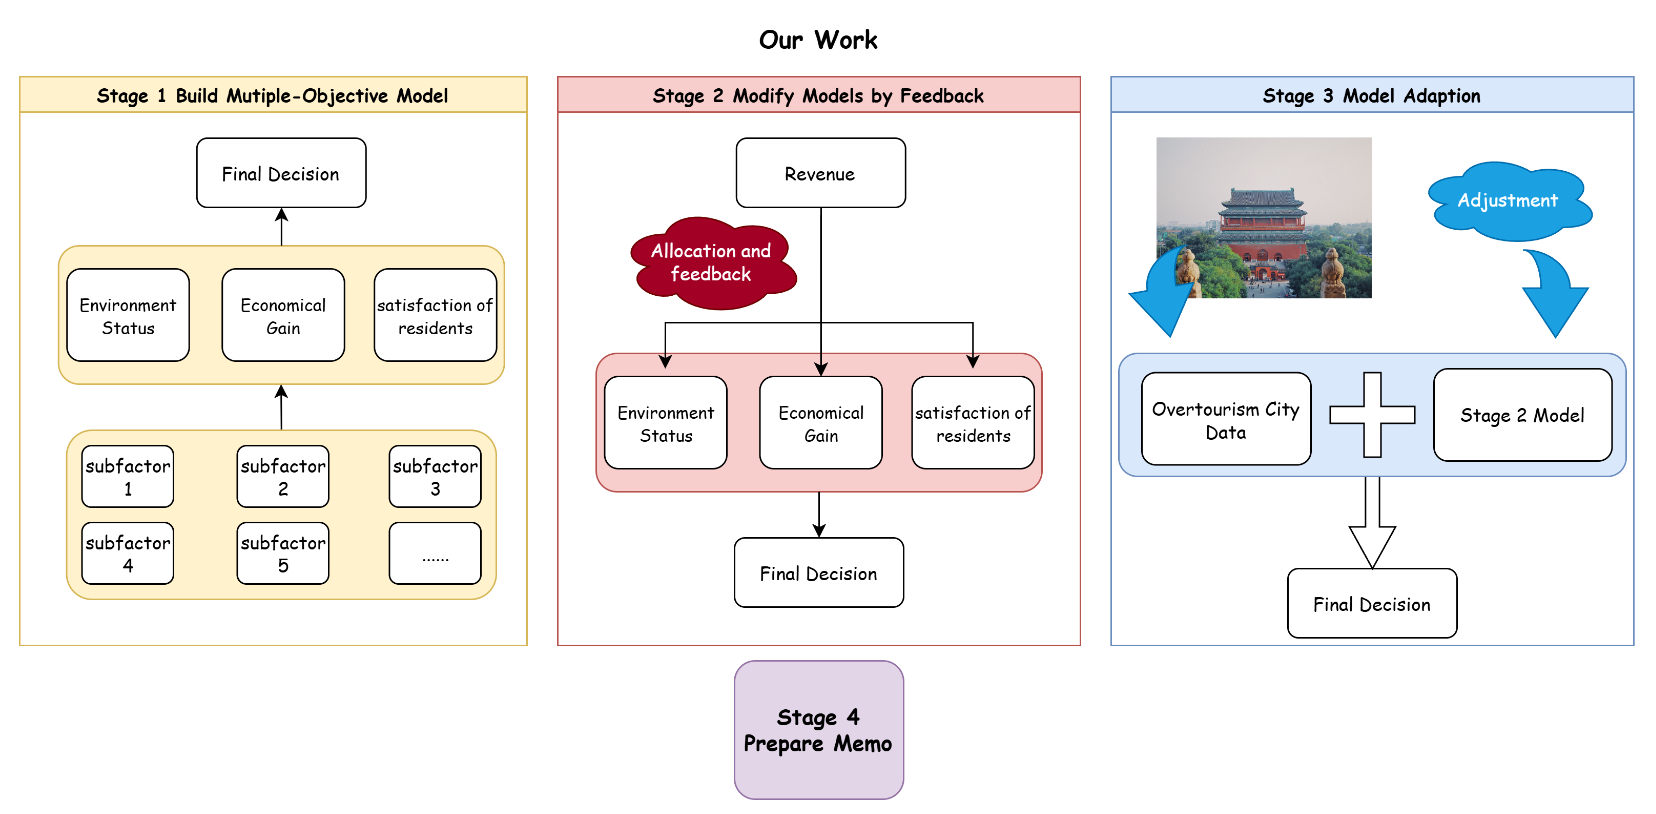
\includegraphics[width=18cm]{overview.png}
                \caption{Overview of our works}
            \end{figure}
    \section{Assumptions}

                \hspace*{1em} \textbf{$\bullet$ Assumption 1: Animals naturally increase at the same rate every year.} \\
                \hspace*{2em} \(\Rightarrow\) \textbf{Justification:} Though the ecnomic growth of the world happens each year, so is the inflation rate growing at a similar rate. What's more, people tend to make budget and have constant consumption habits.\\
                \hspace*{1em} \textbf{$\bullet$ Assumption2: The tourist council can totally control the number of toursists each year but no more than the highest level.} \\
                \hspace*{2em} \(\Rightarrow\) \textbf{Justification:} In this model, we assume that there is always overtourism problem, so the officers of the council can limit the numbers of tourists by issuing polices. It is also a fact that in 2020, no more than 100 people travelled at Juneau.\\
                \hspace*{1em}      \textbf{$\bullet$ Assumtion3: the ratio  of tourists on a cruise ship to the total number of tourists is nearly constant.} \\
                \hspace*{2em} \(\Rightarrow\) \textbf{Justification:} In this model, we disregard the fact that this ratio changes since it is relatively uncorrelated to our proect.\\
                \hspace*{1em}\textbf{$\bullet$ Assumption 4: The data collected can be considered reliable and reflect the state of the natural environment.} 
        \\        \hspace*{2em} \(\Rightarrow\) \textbf{Justification:} we searech for data from reliable resoucres with high accuracy.
    \section{Notations and Description}
        \hspace*{2em}Important notations used in this paper are listed in the table 1.
        \vspace{-.5em}
        \begin{table}[htbp]
            \centering
            \caption{Notations}
            \vspace{0.5em}
            \begin{tabular}{cc}
                \toprule                % 顶部线
                    \textbf{Symbols} & \textbf{Description} \\ 
                \midrule                % 中部线
                $I$        & Total tourism revenue of Juneau every year \\ 
                $V$        & The total number of tourists every year \\ 
                $s$        & Per capita spending by tourists \\ 
                $r$        & tax rate related to tourism \\  
                $B$        & Additional revenue of tourism \\ 
                $E$        & Environmental status, as indicated by glacier area \\ 
                $\mu$      & Environmental damage per dollar spent by tourists \\ 
                $\delta$   & Self-healing coefficient of the environment  \\ 
                $g$        & Environmental governance effect per dollar used by government \\ 
                $k$        & Proportion of additional revenue invested in glacier protection \\ 
                $G$        & Economic gain \\ 
                $a$        & Jobs created per tourist \\ 
                $S$        & Resident Satisfaction \\  
                \bottomrule             % 底部线
            \end{tabular}

        \end{table} \\
        \hspace*{2em} Note: Some variables not listed here will be described in their section.


        \section{Model Preparation}
        \subsection{Data Collection}
        \hspace*{2em}the data in reference is only relevant to cruise, so finding available and reliable data is one of the most important part of the research. Through the analysis of our mathematical model, we collected statistic about the tourism of Juneau, including per tourist consumption , Component analysis of consumption per tourist and other data. In addition, we also collect results of Survey of the Local Population on Tourism and Natural conditions such as local temperature, humidity and data related to glacial melting.
        \begin{table}[htbp]
            \centering
            \caption{Data source collation}
            \vspace{0.5em}
            \begin{tabular}{ccc}
                \toprule                % 顶部线
                    \textbf{Data Description} & \textbf{Data Resources} & \textbf{Types} \\ 
                \midrule                % 中部线
                $Tourism Data$        & https://juneau.org    &  Economy                \\ 
                $Environment Data$        & https://datacommons.org/  & Environment\\ 
                $Alaska Glacier Data$        & https://www.nps.gov   & Environment\\ 
                \bottomrule             % 底部线
            \end{tabular}
            \label{tab:notations}
        \end{table}
        \subsection{Data Cleaning}
        \hspace*{2em}We conducted rigorous data cleaning to ensure the accuracy and reliability of our analysis. One specific example involved addressing the anomalous tourist numbers for Juneau during 2020 and 2021. These years experienced a dramatic drop in tourist arrivals due to the COVID-19 pandemic, which introduced outliers that did not reflect typical tourism patterns.
        \begin{figure}[htbp]
            \centering
            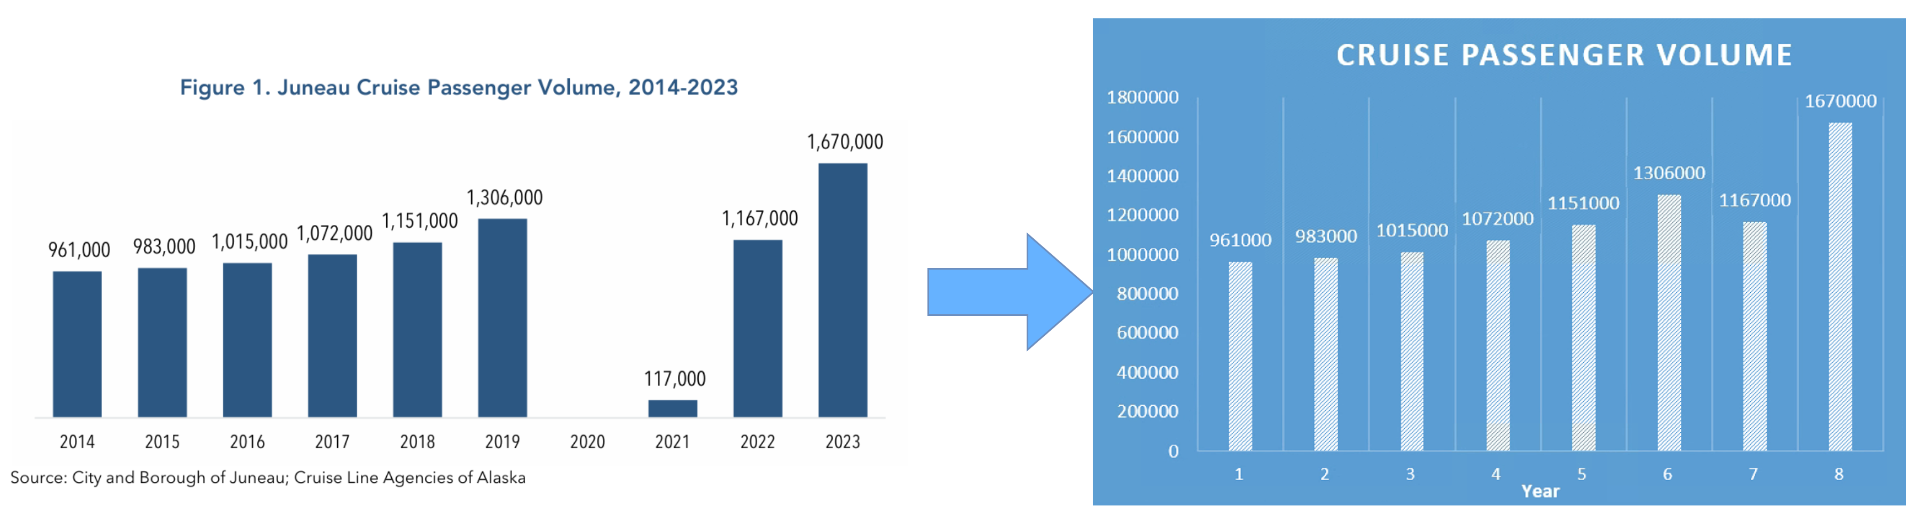
\includegraphics[width=16cm]{dataclean.png}
            \caption{Data cleaning example}
        \end{figure}

        \subsection{Data Standardization}
        \hspace*{2em}Since the model incorporates multiple features, such as the number of tourists, tourism revenue, environmental impact indicators, and policy parameters, these variables operate on vastly different scales. To address this, we applied standardization steps. For example, continuous variables, such as the number of tourists {$V$}, revenue {$I$}, and glacier area {$E$}, were normalized using the Min-Max Scaling method:
        \begin{equation}
        \begin{aligned}
            {X}' = \frac{x-x_{min}}{x_{max}-x_{min}} 
        \end{aligned}
        \end{equation}
        \hspace*{2em} This ensures that all values are scaled between 0 and 1, preserving their relative distribution.


    \section{Multi-objective Optimization Model}
    \hspace*{2em}based on the Objective 1 and Objective 2, we establishes the multi-objective strategy selection model to determine how the number of tourists, the tax rate, and the distribution of additional revenue should be adjusted to get the best outcomes.
    \subsection{Model Structure}
    \hspace*{2em} We establish a 3-layer multi-objective optimization model using Sequential Least Squares Programming (SLSQP) Algorithm to maximize the final score considering 3 factors, also as our  evaluation indicators. They are ecnomic gain {$G$}, environemnt status {$E$}, and satisfaction of residents {$S$}. The Following Figure shows our model structure. The factors with underline are optimize factors.
    \begin{figure}[htbp]
        \centering
        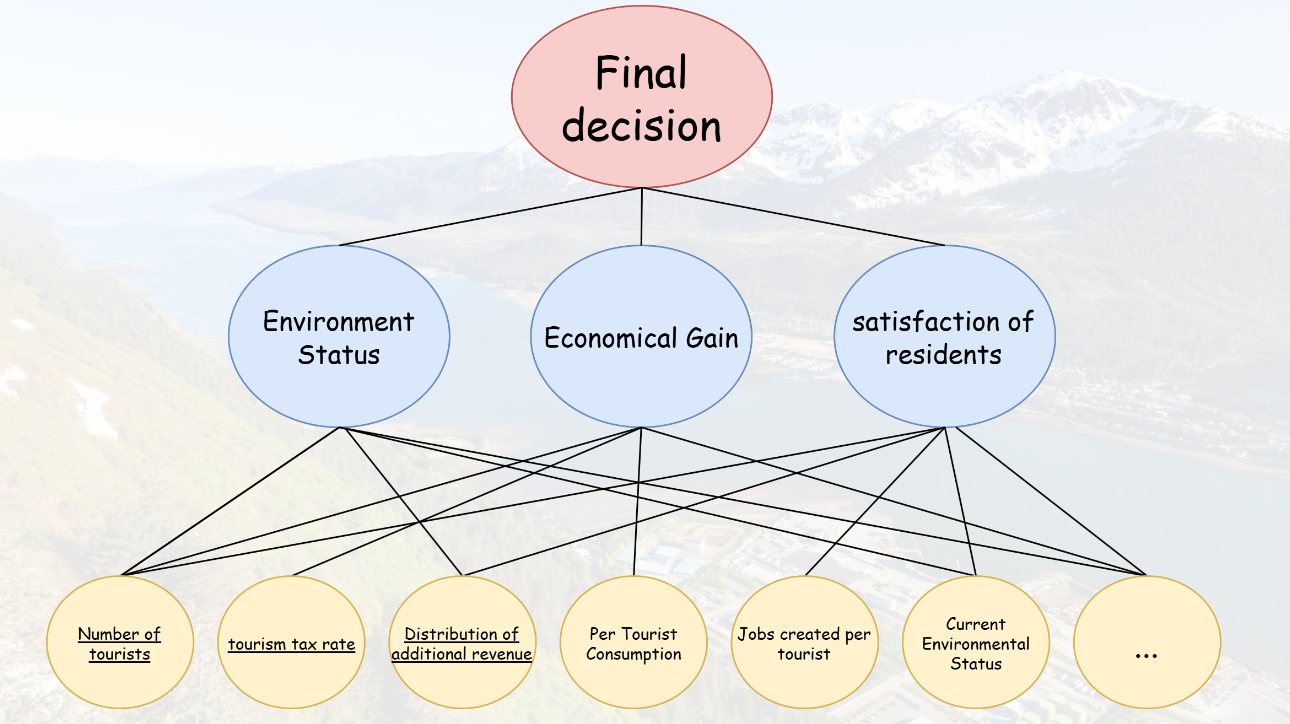
\includegraphics[width=16cm]{multiobjective.png}
        \caption{Our Multi-objective Optimization Model Overview}
    \end{figure}\\
    \hspace*{2em} The figure illustrates the flowchart of our strategy evaluation model, consisting of 3 layer. Here is further explanation of these layer:
    \\ \hspace*{2em} \textbf{Layer 1:} The first layer is the ultimate goal of the model, i.e. to make decisions on the integrated sustainable development of a tourist destination, and balances these factors by taking into account environmental protection, economic gains and resident satisfaction.
    \\ \hspace*{2em} \textbf{Layer 2:} The second layer represents the three key evaluation objectives that influence the final decision, which are calculated from the specific decision variables and data inputs in the third layer, respectively. We will discuss them in their respective segments
    \\ \hspace*{2em} \textbf{Layer 3:} The layer includes all the variables that affect the core indicators and is divided into two categories:
    \\\hspace*{2em}Decision variables:
    These are the variables that we can adjust to optimize the final decision.
    \\\hspace*{2em}Data inputs:
    These are external input data to the model that reflect the current state.
    
    Then we will demonstrate model building steps to calculate layer 2 indicators, and then the process of SLSQP.
    
    \subsection{Building Models for Layer 2 Indicators}
    \subsubsection{Environment Status Model}
    
    \hspace*{2em} \textbf{Given Objectives 1 and 2}, this paper translates the conflict between \textbf{overtourism} and \textbf{natural preservation} into the optimization of the relationship model, referred to as the \textbf{Tourists-Tax-Environment Model}.
    
    \textbf{Firstly}, we introduce some intermediate variables for clear explanation. Based on \textbf{Assumption 1}, the total tourism revenue of Juneau (\(I\)) is fully dependent on the number of tourists (\(V\)). \textbf{Furthermore}, to generate additional revenue for city management and to promote sustainable development, the Council of Tourism has enacted measures to levy a tax at a rate of \(\tau\), resulting in additional revenue (\(B\)).
    

    \begin{equation}
        \begin{aligned}
        {I} = {V}  \times {s}
        \end{aligned}
        \end{equation}
        \begin{equation}
            \begin{aligned}
{B} = \frac{I r}{1+r}
            \end{aligned}
            \end{equation}

        Here $s$ denotes Per capita spending by tourists.
        
        \hspace*{2em} \textbf{Next}, we estimate the \textbf{footprint of tourists} based on their actual consumption, which is calculated as the difference between the total tourism revenue (\(I\)) and the additional revenue (\(B\)). 

        It has been reported that the rate at which \textbf{Mendenhall Glacier} was melting was significantly high from 2014 to 2019. This indicates that the glacier has lost its ability to self-recover, and the rate of melting accelerates as the glacier continues to shrink. Let \(E\) denote the area of \textbf{Mendenhall Glacier}.
        

\begin{equation}
    \begin{aligned}
\frac{\text{d}E}{\text{d}t}  =  \mu \frac{I}{1+r}+\delta E 
    \end{aligned}
    \end{equation}

    Where we succesfully estimated the natrual conservation status by ${E}$.

Secondly, consider the expenditures from additional revenue the tourist council spend for preserving environment , with a effective rate ${g}$, Our model can be modified into:

\begin{equation}
    \begin{aligned}
{E_{i+1}} -E_{i} = \mu \frac{I}{1+r} + \delta {E_{i}} +gkB
    \end{aligned}
    \end{equation}

    Clearly, in this dynamical system, consistent decrease of {$E_i$} is avoided,{$E_i$}
   will finally converge at 

   \begin{align*}
    -\frac{(\mu  + gkr)I}{\delta(1+r)}
            \end{align*}


            \subsubsection{Economic Gain Model}

            \hspace*{2em} We propose the following simplified model to estimate the \textbf{economic gain} (\(G\)) by the total number of jobs created for residents. One of our references \cite{Xu} has demonstrated that the economic gain of a city (\(G\)) has a \textbf{linear relationship} with the number of tourists every year (\(V\)).
            

    \begin{equation}
        \begin{aligned}
        G = Va
        \end{aligned}
        \end{equation}

        Based on ${Cruise impact report of Juneau}$. we can conclude that for Juneau, $a$ = 0.00230538.


        \subsubsection{Satisfaction of Residents Model}

        \hspace*{2em} Once the models for \textbf{environmental status} and \textbf{economic gain} were established, it becomes possible to compute the \textbf{index of satisfaction of residents}. This index can later serve as a \textbf{constraint}, enabling a more comprehensive evaluation of sustainable tourism by balancing the needs of both \textbf{residents} and \textbf{tourists}. Moreover, it can also act as an indicator of \textbf{the degree of city development}.
        



    Resident satisfaction can be regarded as a linear combination of the above three variables:

    \begin{equation}
        \begin{aligned}
S = \alpha E+\beta G +\gamma(1-k)B
        \end{aligned}
        \end{equation}

        where $\alpha$, $\beta$, and $\gamma$ are the weights of the three factors, respectively. Their values can be obtained from similar studies\cite{Cottrell}: $\alpha = 0.34$, $\beta = 0.46$, and $\gamma = 0.2$.


        \begin{figure}[htbp]
            \centering
            \begin{minipage}{0.45\textwidth}
                \centering
                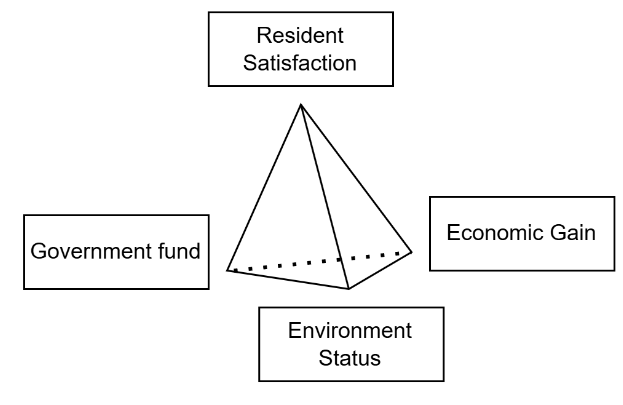
\includegraphics[width=\textwidth]{pyramid.png}
                \caption{The Pyramid of Satisfaction of Residents}
            \end{minipage}\hfill
            \begin{minipage}{0.45\textwidth}
                \centering
                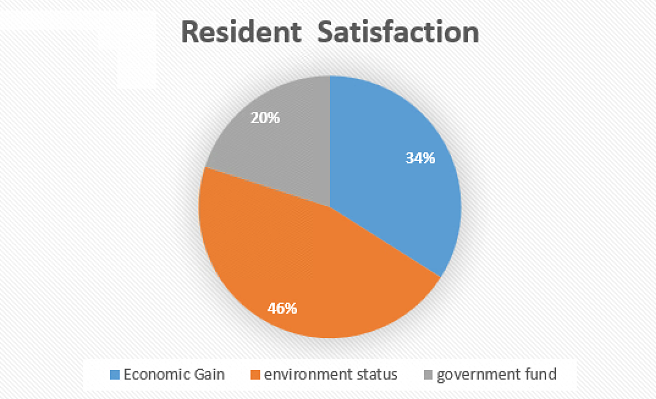
\includegraphics[width=\textwidth]{circle.png}
                \caption{Ratio of Components of resident satisfactions}
            \end{minipage}
        \end{figure}

        Figure 5 shows the components of resident satisfaction, which are the three factors we have discussed above. Figure 6 shows the ratio of the three components obtained from the reference\cite{Cottrell}.

        \subsection{Multi-objective Optimization Model}
        \subsubsection{Optimization problems}
        \begin{enumerate}
            \item \textbf{Objective function:} \\
            \hspace*{2em}Maximize the negative value of the weighted score (since minimize is a minimization algorithm):

            \begin{equation}
                \begin{aligned}
        objective = - (0.5\times bar(E)+0.5\times bar(G))
                \end{aligned}
                \end{equation}

                where $bar(X)$ is the normalization function that normalizes $X$ to the interval [0, 1]. We chose the maximum value of local glacier area since the beginning of the record as ${E_{max}}$, the ....... as ${E_{min}}$, the ......... as ${G_{max}}$, and the ....... as ${G_{min}}$

            \item \textbf{Constraints:} \\
            \begin{align*}
                Satisfaction & \geq 0.5 
            \end{align*}
            \begin{equation}
                \begin{aligned}
        constraint=S(E,G,B,k)-0.5
                \end{aligned}
                \end{equation}

                where S is a composite score function to measure sustainable development, shown below:

                \begin{equation}
                    \begin{aligned}
            S=a\times bar(E)+b\times bar(G)+c\times (1-k)\times B
                    \end{aligned}
                    \end{equation}

         \item \textbf{Variable boundaries:} \\
                \[
        0 \leq I \leq I_{\text{max}}, \quad 0 \leq r \leq r_{\text{max}}, \quad 0 \leq k \leq k_{\text{max}}
        \]

        then we can calculate the boundaries of $E$, $G$, $B$, $S$.\\
        To calculate the boundaries of E,we use the value method finds its maximum and minimum values. The visualized result is shown in the figure, where the X-axis is $I$, the Y-axis is $r$ and the z-axis is $k$
        
        \begin{figure}[htbp]
            \centering
            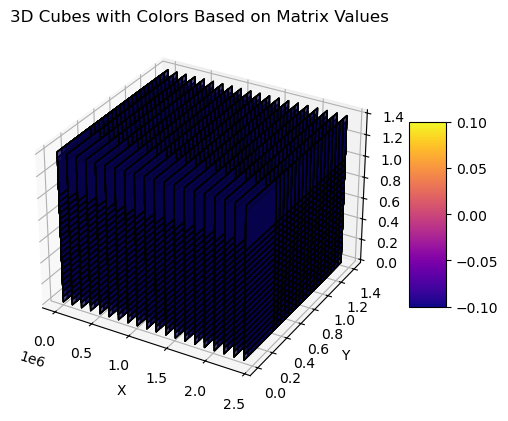
\includegraphics[width=12cm]{cube.png}
            \caption{HOWTONAMETHIS}
        \end{figure}
    
        \begin{table}[htbp]
            \centering
            \caption{HOWTONAMETHIS}
            \begin{tabular}{lcccc}
                \toprule
                & \textbf{B} & \textbf{E} & \textbf{G} & \textbf{S} \\
                \midrule
                \textbf{max} & 2,394,779 & 54,581.723 & 1,197,390 & 1 \\
                \textbf{min} & 0 & -15,096.465 & 0 & 0 \\
                \bottomrule
            \end{tabular}
            \label{tab:data_summary}
        \end{table}      
        \end{enumerate}

        \subsubsection{Optimization process}

        \begin{itemize}
            \item \textbf{Initial Estimate:} 
            \[
            x_0 = \left[ \frac{I_{\text{max}}}{8}, \frac{r_{\text{max}}}{1.4}, \frac{k_{\text{max}}}{6.5} \right]
            \]
            \item \textbf{Solution:} Optimize the objective function using the SLSQP method while satisfying the constraint \( S \geq 0.5 \).
            \item \textbf{Outputs:}
            \begin{itemize}
                \item Optimal total tourism revenue  \( I_{\text{opt}} \).
                \item Optimal tourist spending ratio \( r_{\text{opt}} \).
                \item Optimal proportion of environmental governance inputs \( k_{\text{opt}} \).
                \item Optimal state of the environment \( E_{\text{opt}} \).
                \item Optimal economic return \( G_{\text{opt}} \).
                \item Composite Sustainability Score \( S_{\text{opt}} \).
            \end{itemize}
        \end{itemize}
        
        \begin{table}[htbp]
            \centering
            \caption{Optimal Values of Variables}
            \begin{tabular}{lc}
                \toprule
                \textbf{Variable (\( \text{opt} \))} & \textbf{Optimal Value} \\
                \midrule
                \( I_{\text{opt}} \) & 299,347.50000704837 \\
                \( r_{\text{opt}} \) & 0.124 \\
                \( k_{\text{opt}} \) & 0.999 \\
                \( E_{\text{opt}} \) & 34.658 \\
                \( S_{\text{opt}} \) & 0.512 \\
                \bottomrule
            \end{tabular}
            \label{tab:optimal_values}
        \end{table}
        
        \subsection{Predictions by the model}

        The figure below shows the comparison of glacier area before and after optimization. Based on our model, the glacier will totally disappear in 60 years if no measures are taken. However, with the optimal management strategy, the glacier area will be preserved at a sustainable level.
        \begin{figure}[htbp]
            \centering
            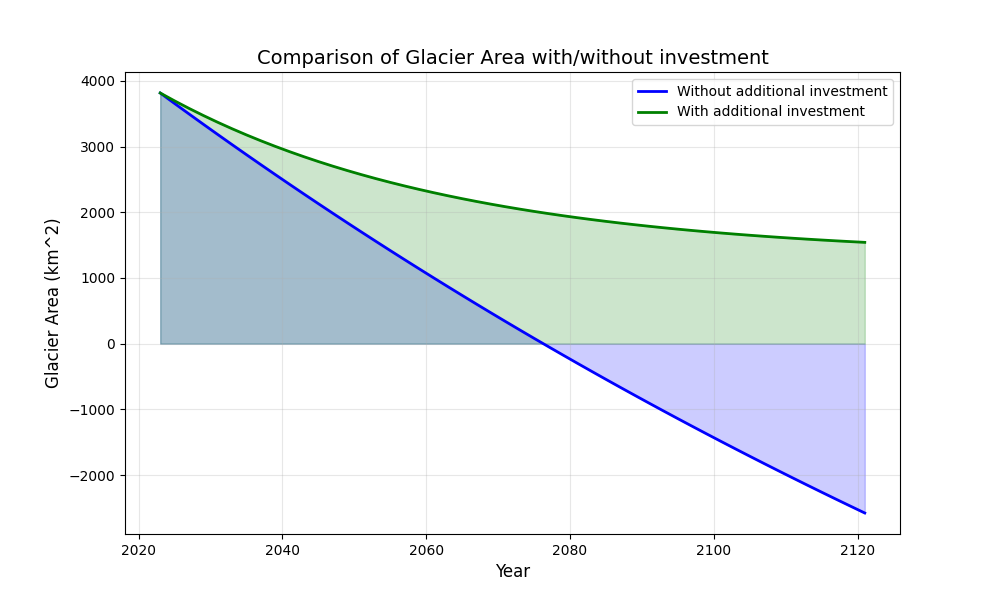
\includegraphics[width=18cm]{predict.png}
            \caption{Comparison of glacier area before and after optimization}
        \end{figure}
        \subsection{Sensitivity Analysis}
        \hspace*{2em}To analyze the function \( E \) with regard to \( I \), \( r \), and \( k \), we need to calculate the partial derivatives of the function with respect to these variables and visualize these sensitivities.

        Given the function \( E \) as follows:
        \begin{equation}
            \begin{aligned}
            E = -\frac{(\mu + gkr)I}{\delta(1 + r)}
            \end{aligned}
            \end{equation}
            
        The partial derivatives are:

        1. Partial derivative with respect to \( I \):
        \begin{equation}
            \begin{aligned}
            \frac{\partial E}{\partial I} = -\frac{\mu + gkr}{\delta(1 + r)}
            \end{aligned}
            \end{equation}
        \hspace*{2em}2. Partial derivative with respect to \( r \):
        \begin{equation}
            \begin{aligned}
            \frac{\partial E}{\partial r} = -\frac{(\mu + gkr)I}{\delta(1 + r)^2} + \frac{gkI}{\delta(1 + r)}
            \end{aligned}
            \end{equation}

        3. Partial derivative with respect to \( k \):
        \begin{equation}
            \begin{aligned}
            \frac{\partial E}{\partial k} = -\frac{gIr}{\delta(1 + r)}
            \end{aligned}
            \end{equation}
    
            We analyzed each of these parameters to explore the impact of \textbf{total tourism revenue}, \textbf{tax rates}, and the \textbf{portion of tax allocated to environmental protection} on an economic or environmental indicator.

            In this analysis, we first fixed the tax rate and the {proportion of investment in environmental protection} at their optimal values. We then allowed the \textbf{total tourism income} to vary between 0 and 50,000, calculating the corresponding economic or environmental index values. \textbf{Secondly}, we fixed the {proportion of total tourism income} and the investment in environmental protection at their optimal values, allowing the {tax rate} to vary between 0 and 0.6, and calculated the corresponding index values. \textbf{Finally}, we fixed the {total tourism income} and {tax rate} at their optimal values, letting the {proportion of environmental protection investment} vary between 0.95 and 1, and calculated the index values.
            
            For each parameter change, we plotted the relationship between the parameter value and the corresponding economic or environmental indicator value to visually demonstrate the interaction between these variables.
            


            \begin{table}[htbp]
                \centering
                \caption{Optimal Values of Variables}
                \begin{tabular}{cc}
                    \toprule
                    \textbf{Variable} & \textbf{Optimal Value} \\ 
                    \midrule
                    \( I \) & 299347.5 \\ 
                    \( r \) & 0.124 \\ 
                    \( k \) & 0.999 \\ 
                    \bottomrule
                \end{tabular}
                \label{tab:optimal_values}
            \end{table}

            \begin{figure}[htbp]
                \centering

                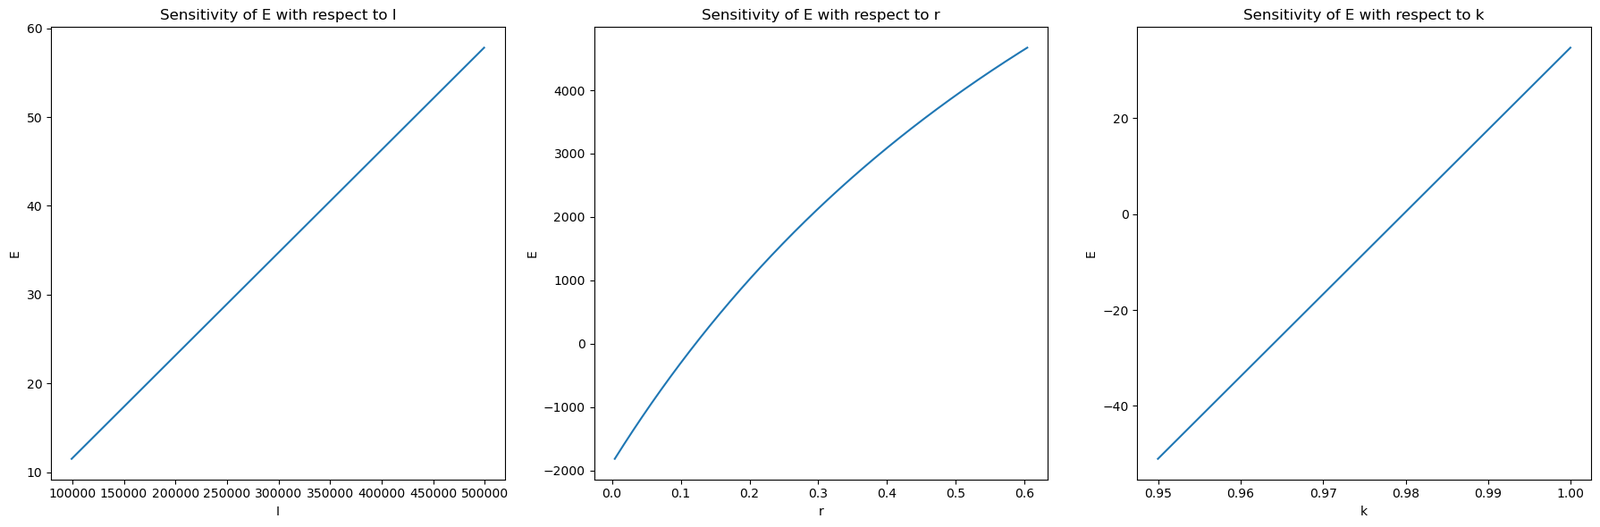
\includegraphics[width=16cm]{threelines.png}
                \caption{Sensitivity Analysis of different variables}
            \end{figure}
            
            

    \section{Adapting Sustainable Tourism Models to Address Overtourism}
            \subsection{Introduction}
            \hspace*{2em}Beijing, the capital of China, a city steeped in history and culture, was once mired in the smoggy haze that obscured its skyline and compromised the health of its residents. The air quality was a pressing concern, not only for the locals but also for the millions of tourists who flocked to the city each year. However, thanks to the government's proactive measures and relentless efforts, Beijing now boasts clean blue skies, a testament to the city's dedication to environmental improvement.
                        
            The Air Quality Index (AQI) is a crucial tool for communicating air pollution levels and health risks in Beijing. It's based on concentrations of pollutants like PM2.5, O3, NO2, SO2, and CO. The AQI is categorized from "Good" to "Hazardous," helping residents and visitors make informed decisions about outdoor activities. By monitoring the AQI and taking precautions like staying indoors on high-pollution days, the public can protect their health. Together with government measures, the AQI contributes to cleaner air and healthier living in Beijing.

            \begin{figure}[htbp]
                \centering
                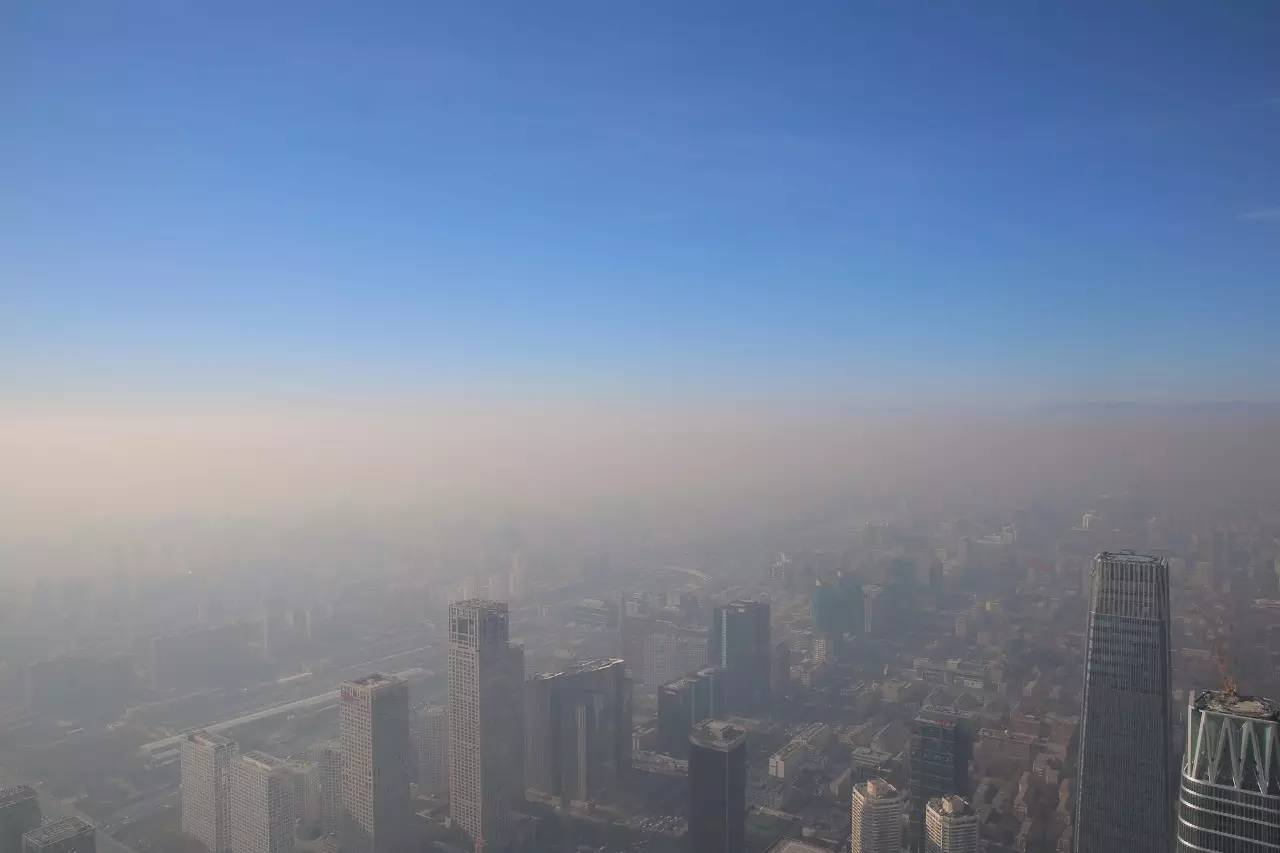
\includegraphics[width=8cm]{smog.png}
                \caption{Beijing smog}
            \end{figure}

            \subsection{Model Adaptation}
            \hspace*{2em}model implement process:
            \begin{enumerate}
                \item \textbf{Determine the calculation method of environmental assessment index} \\
                \hspace*{2em}For Beijing we choose AQI as Environmental assessment index $E$ (which is obtained by intuition) and the $\mu$ and $\delta$ parameters in the formula, which is by using previous years' data.

                \begin{table}[htbp]
                    \centering
                    \caption{Beijing Environmental Assessment Data (2017-2023)}
                    \begin{tabular}{cccc}
                        \toprule
                        \textbf{Year} & \textbf{\( V \) (Ten thousands of people)} & \textbf{\( I \) (Hundred million yuan)} & \textbf{AQI} \\ 
                        \midrule
                        2023 & 32853.7 & 5849.7  & 82.33 \\ 
                        2022 & 18230.8 & 2520.26 & 73.67 \\ 
                        2021 & 25512.8 & 4166.2  & 77.92 \\ 
                        2020 & 18386.5 & 2914.0  & 78.58 \\ 
                        2019 & 32209.8 & 6224.6  & 86.50 \\ 
                        2018 & 31093.6 & 5921.2  & 87.00 \\ 
                        2017 & 27463.9 & 4934.3  & 81.70 \\ 
                        \bottomrule
                    \end{tabular}
                    \label{tab:beijing_env_data}
                \end{table}
                


                \item \textbf{Calculate $B$, $E$, $G$, $S$ range}
                \\ \hspace*{2em}similiar to the above, we use the value method to calculate the boundaries of $E$. The visual result is shown in the figure:

                \begin{figure}[htbp]
                    \centering
                    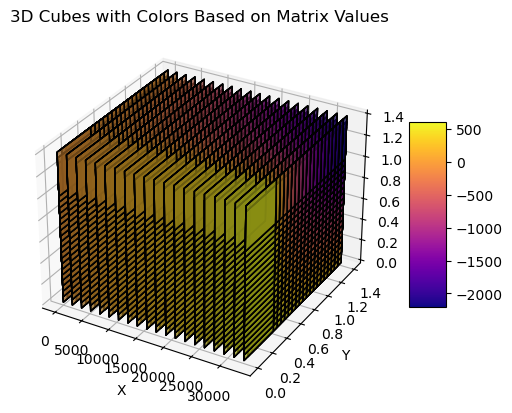
\includegraphics[width=12cm]{cube2.png}
                    \caption{HOWTONAMETHIS}
                \end{figure}
                
                \begin{table}[htbp]
                    \centering
                    \caption{HOWTONAMETHIS}
                    \begin{tabular}{lcccc}
                        \toprule
                        & \textbf{B} & \textbf{E} & \textbf{G} & \textbf{S} \\
                        \midrule
                        \textbf{max} & 2,394,779 & 54,581.723 & 1,197,390 & 1 \\
                        \textbf{min} & 0 & -15,096.465 & 0 & 0 \\
                        \bottomrule
                    \end{tabular}
                    \label{tab:data_summary}
                \end{table}
                
                \newpage
                \item \textbf{Use the same optimization algorithm to get the optimal solution.} 
                \\
                \hspace*{2em}By applying Weighting method and SLSQP algorithm, we can analysis what to do according to numerical results. In this problem we can get several strategies to balance the Tourism and smog problem in Beijing:
                \begin{enumerate}
                    \item[(a)] Limit the number of visitors.
                    \item[(b)] Lower taxes.
                    \item[(c)] Improve the structure of government investment in environmental protection.
                    \end{enumerate}


                    \begin{table}[htbp]
                        \centering
                        \caption{Optimal Values of Variables}
                        \begin{tabular}{l c}
                            \toprule
                            \textbf{Variable} & \textbf{Optimal Value} \\
                            \midrule
                            \( I \) & 1716.494 \\
                            \( r \) & 0.0193 \\
                            \( k \) & 0.801 \\
                            \( E \) & 31.410 \\
                            \( S \) & 0.5 \\
                            \bottomrule
                        \end{tabular}
                        \label{tab:optimal_values}
                    \end{table}
                \end{enumerate}
                \subsection{Impact of Location-Specific Factors}

                \hspace*{2em} \textbf{Comparing} the models of Beijing and Juneau, the main ecological problems are different, which leads to the selection of distinct environmental assessment indices. Beijing, located inland and serving as the economic and political center of China, is an international metropolis. Its ecological problems differ significantly from those of Juneau, a tourist city. The selection of \textbf{haze} as the evaluation index for Beijing and \textbf{iceberg area} as the evaluation index for Juneau is based on their distinct ecological characteristics.
                
                \begin{figure}[htbp]
                    \centering
                    \begin{minipage}{0.45\textwidth}
                        \centering
                        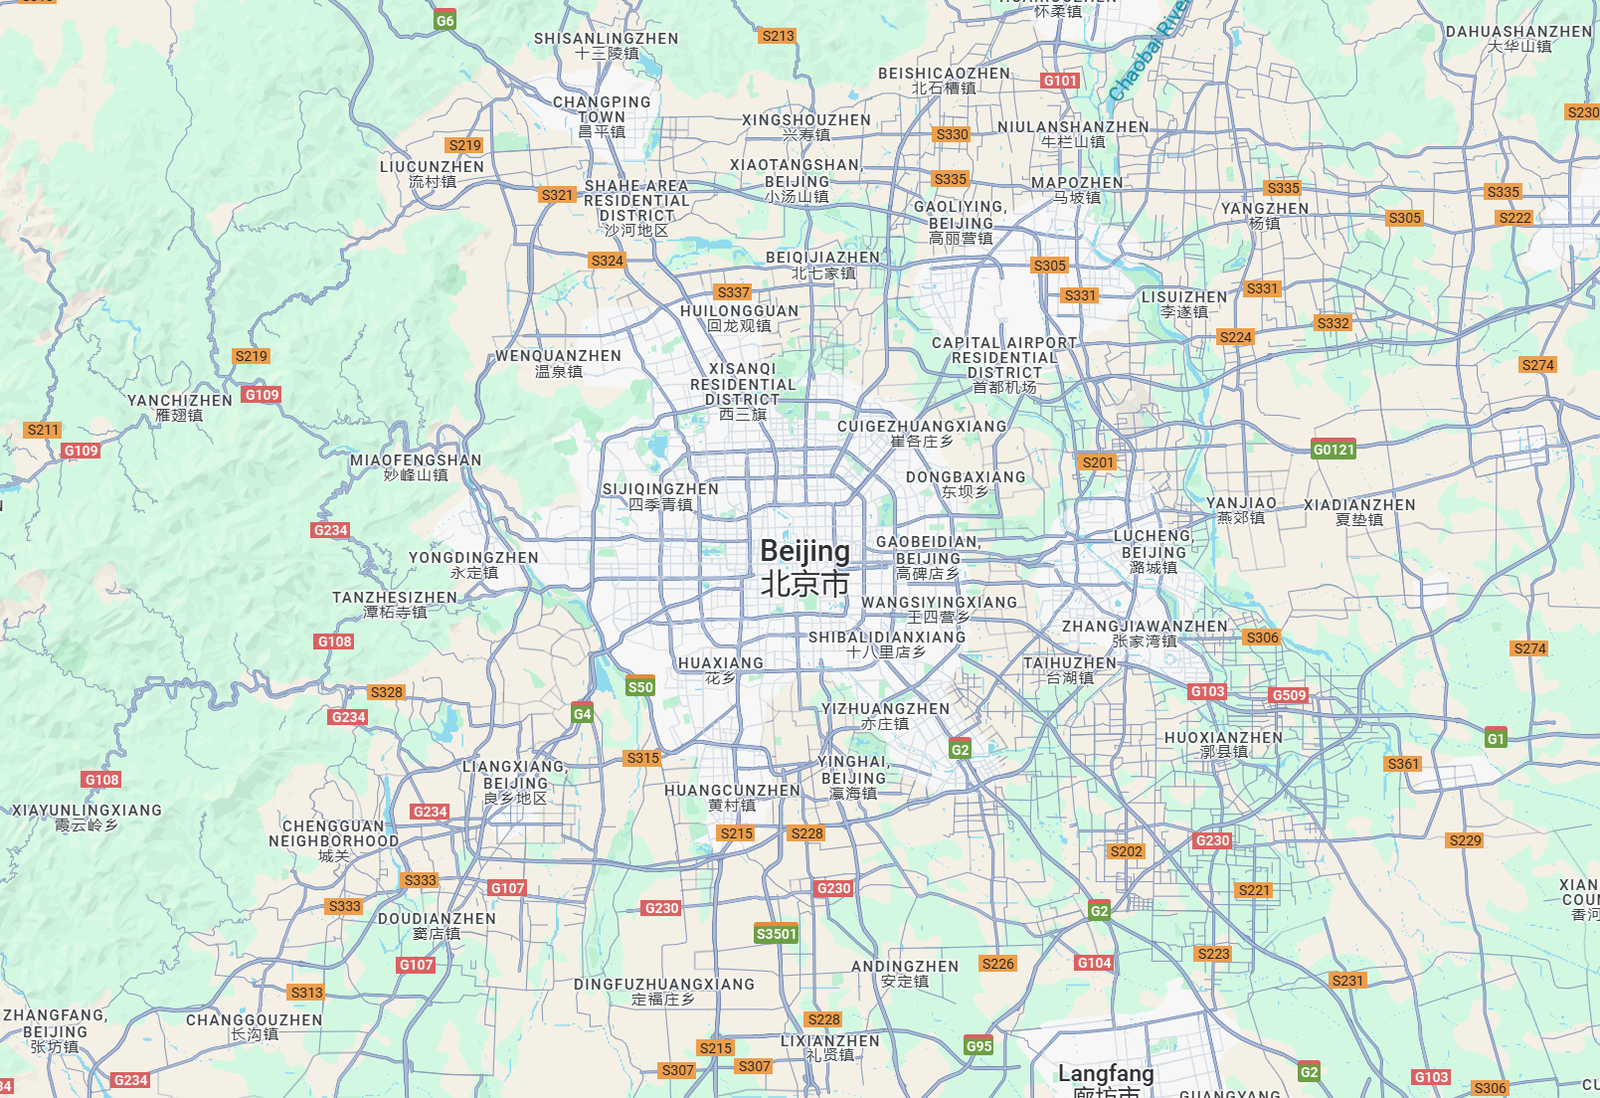
\includegraphics[width=\textwidth]{map1.png}
                        \caption{Map of Juneau}
                    \end{minipage}\hfill
                    \begin{minipage}{0.45\textwidth}
                        \centering
                        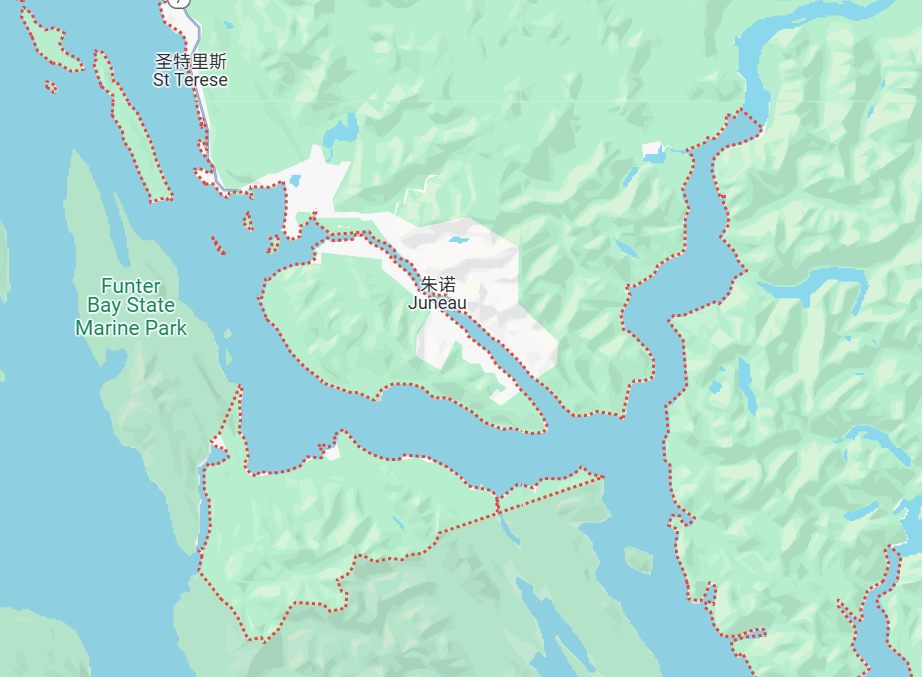
\includegraphics[width=\textwidth]{map2.png}
                        \caption{Map of Beijing}
                    \end{minipage}
                \end{figure}
                
    \textbf{In addition}, the differing tourism industries of the two cities also lead to variations in their ecological damage and protection priorities. Tourism in Juneau primarily involves \textbf{natural attractions}, such as whale watching and glacier scenery, requiring consideration of tourists' direct interaction with the ecology. By contrast, tourism in Beijing is largely focused on the \textbf{tertiary industry}, where tourists indirectly impact the environment through commodity consumption. 
                
\textbf{Therefore}, different strategies are applied for the consideration of variable \(k\): in Juneau, direct protection is emphasized, such as banning littering and limiting the number of whale watchers, and the value of \(k\) should be set relatively high. For Beijing, tax revenue should not be directly invested in environmental protection, and the \(k\) value should be relatively low.
                
            \subsection{Promoting Balance}
            1145141919810

            072107210721
            \section{Conclusion}
            \subsection{Summary of Results}

 \textbf{$\bullet$ Objective 1}\\ 
            \hspace*{2em} We established tourist-revenue-environment coupling model, processed the data to get coefficient and predicted the area of the galcier in Alsaka based on a dynamic system model.
            If the goverment would not take additional revenue and limit the growth of number of tourists, the area of the glacier will decrease at a groing rate. However, due to pervious report of officially fund for natural preversation, a promising and obvious contain can be persued.\\
   \textbf{$\bullet$ Objective 2}\\ \hspace*{2em} Objective Based on multiple objective optimization model. First, strategies and policies that can be optimized has been simplified to the number of tourists, the distribution of additional revenue.Multi-objective optimization model is proposed to quantify the economic and ecological impacts of an optimal combination of strategies and policies.
            We finally get the suggested solution for idealed predictions.\\
     \textbf{$\bullet$ Objective 3}\\
            \hspace*{2em} We demonstrated how the developed model can be adapted to other tourist destinations impacted by overtourism.
            

    \section{Model Evaluation}
        \subsection{Strengths}
        \begin{enumerate}
\item The model incorporates economic, ecological and social factors, and examines the  sustainable development of sustainable tourism from different subjects, like the satisfaction of local residents, the environmental.
																																																																																				
\item This model shows high replicablilty . We pointed out general factors and indices for over-tourism cities, as well as long-term predictions. It can even be applied to ecosystems, to consider the sustainable development for the whole society.
\end{enumerate}

            
        \subsection{Weaknesses}
            \begin{enumerate}
                \item \textbf{Weakness: }The number of factors we consier is relatively small, which may not fully refelct the actual world with complexity.\\
                \hspace*{2em} \textbf{Improvement:} In order to simplify the model, we consider a small number of factors. In fact, it is a better way to seperate different kinds of overtourism cities into different typres, different indices to estimate the environment conditions,to make the model more satisfied with the actual condition.
            \end{enumerate}


    %\label{LastPage2}
    \addcontentsline{toc}{section}{References}
    \begin{thebibliography}{99}

        \bibitem{Xu}
        Xu H., Bao H.: On the methods of ecological security design for nature reserves [J]. The Journal of Applied Ecology, 2004, 15(7): 1266-1270.
        \bibitem{Liang}
         Liang C., Li X.: The ecological sensitivity evaluation in yellow river delta national natural reserve [J]. Soil, Air, Water, 2012, 40(10): 1197-1207.
        \bibitem{zhu}
        Zhu S., Kong X.,:et al. Identification of the human-land relationship involved in the urbanization of rural settlements in Wuhan city circle, China [J]. Journal of Rural Studies.
        \bibitem{Yuan}
        Yuan G.:The positive interaction between industrial development, people's well-being, and local government governance - a discussion on the value of the happiness index of residents in tourist destinations,[J]. Theory introduction,2012,(09)89-91.
        
        \bibitem{Thomas}
        Thomas D M., Ciesla A., et al.: A mathematical model of weight change with adaptation, [J]. Mathematical biosciences and engineering: MBE, 2009, 6(4): 873.
        
        \bibitem{Davies}
        Davies, B., McNabb, R., Bendle, J. et al.: Accelerating glacier volume loss on Juneau Icefield driven by hypsometry and melt-accelerating feedbacks. Commun,15,5099(2024). 
        
        \bibitem{Tiantian}
        Tiantian G.,Wenjun W.,Fen W.:
        Research on the spatial spillover effect of ecotourism on economic growth - based on data from 60 key tourism cities in China[J]. Ecology and Economic,2024,40(09):127-134.
        
        \bibitem{Cottrell}
        Cottrell, S. P., Vaske, J. J., Roemer, J. M.:
        Resident satisfaction with sustainable tourism: The case of Frankenwald Nature Park, Germany [J].
        Tourism Management Perspectives, 2013, 8: 42-48. 
        DOI: https://doi.org/10.1016/j.tmp.2013.05.005.
        
    
    \end{thebibliography}


    \begin{appendices}
        Here are simulation programmes we used in our model as follow.
        
        \vspace{.5em}
        \noindent(1)\quad \verb|hello.cpp|
        \vspace{.5em}
        \begin{lstlisting}[language = c++, numbers = left]
    #include <iostream>
    int main() {
        std::cout << "Hello, world!\n";
        return 0;
    }
        \end{lstlisting}

    \end{appendices}
    \includepdf[pages={1}]{memo.pdf}

\end{document}
